\documentclass{beamer}
\def\allfiles{}	% 定義主頁,用於單頁編譯辨識用
\usepackage{xeCJK}
\setmonofont[Mapping={}]{JetBrains Mono}
\setmainfont{JetBrains Mono}
\setsansfont{JetBrains Mono}
\setCJKmainfont{微軟正黑體}
\setCJKsansfont{微軟正黑體}
\usetheme[secheader]{Boadilla}
%\usepackage{ctable} % 表格
\usepackage{color} % 字體顏色
\usepackage{hyperref}
\usepackage{listings} % 程式碼區塊用
\lstset{
	language=Java,
	showtabs=false,
	showstringspaces=false
}
\author{Enix Lin}
\begin{document}
	\title{Katalon Studio}
	\subtitle{Regression Testing}
	% 作者放在 document 外面可以去掉告警
	% \author{Enix Lin}
	% \institute{}
	\date{2022/02}
	\maketitle
	%----------------------------
	\begin{frame}[c]
		\label{Index}
		\frametitle{目錄}
		\tableofcontents
	\end{frame}
	%----------------------------
	% 介紹章節
	\ifx\allfiles\undefined
\documentclass{beamer}
\usepackage{xeCJK}
\setmonofont[Mapping={}]{JetBrains Mono}
\setmainfont{JetBrains Mono}
\setsansfont{JetBrains Mono}
\setCJKmainfont{微軟正黑體}
\setCJKsansfont{微軟正黑體}
\usetheme[secheader]{Boadilla}
%\usepackage{ctable} % 表格
\usepackage{color} % 字體顏色
\usepackage{hyperref}
\usepackage{listings} % 程式碼區塊用
\lstset{
	language=Java,
	showtabs=false,
	showstringspaces=false
}
\begin{document}
\input{setting/command}
\fi
%----------------------------
%----------------------------
\section{Introduction}
\begin{frame}
    \frametitle{Introduction}
    Katalon Studio 是一款免費的自動化測試工具,可以安裝在windows、macOS、linux系統上,
    結合了 Eclipse 的部分功能,
    同時可以管理頁面元素、測試資料、測試案例、生成測試報告等功能。~\\
    Katalon Studio 的使用可以用 Eclipse 的操作去適應即可。
    \begin{block}{download link}
        https://www.katalon.com/download/
    \end{block}
    
\includegraphics[width=1\textwidth]{picture/katalonIcon.jpg}
\end{frame}
%----------------------------
\subsection{Quick Start}
\begin{frame}
    \frametitle{Quick Start}
    Katalon Studio 是需要創建 Katalon 帳號方能使用(包含下載也是),
    登入前請先設定好 Proxy。~\\
    以下以內建之導覽範例做簡單介紹。Help => Start Page ~\\~\\
    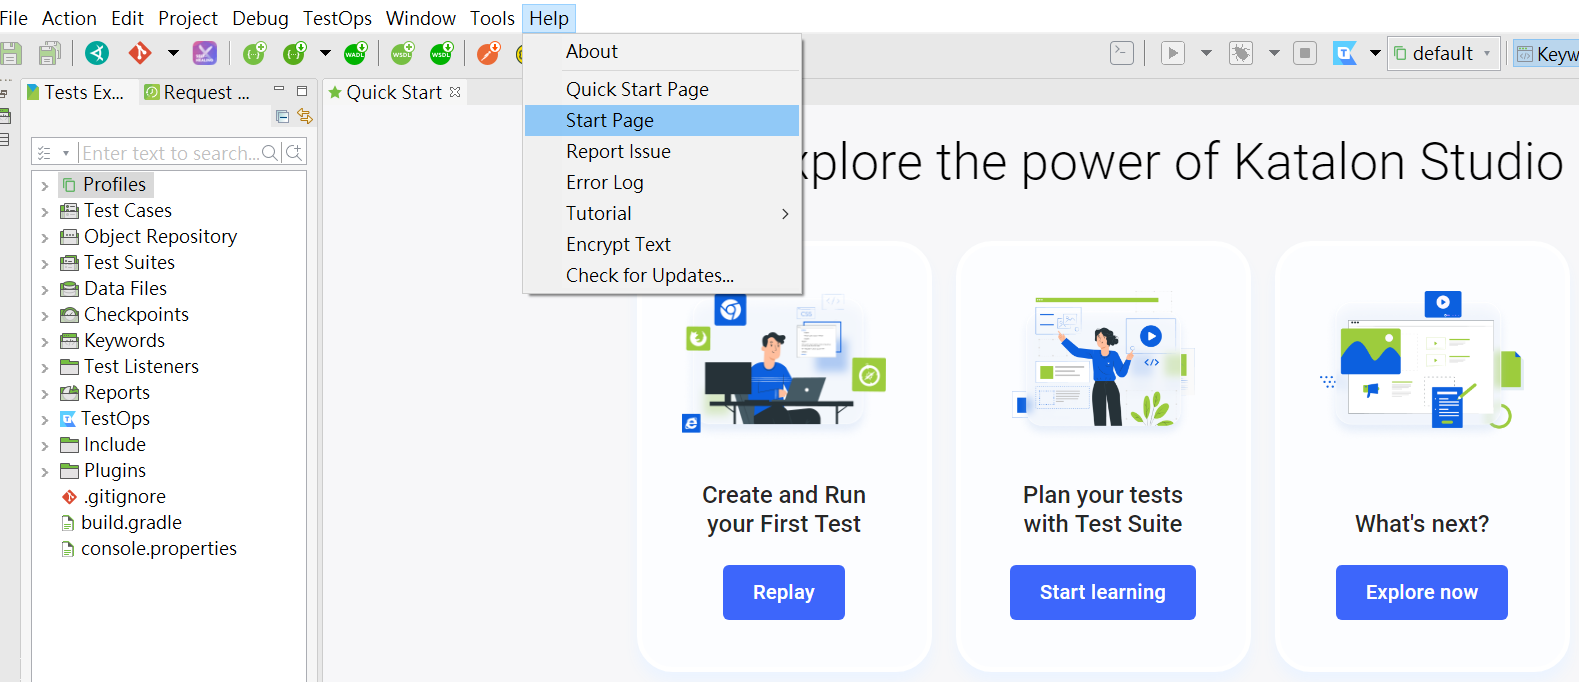
\includegraphics[width=1\textwidth]{picture/quickStart.png}
\end{frame}
%----------------------------
\begin{frame}
    \frametitle{Quick Start}
    由教學可以整理出簡單的結論與順序:
    \begin{enumerate}
        \item 創建 Request 物件,包含設定 URL、Header、Body、自訂變數等
        \item 建立 Test Case Script,將 Request 物件加入
        \item 於 Script 中撰寫驗證規則
        \item 將各 Test Case 組成 Suites 執行
        \item 或再將 Test Case Suites 組成 Collection 執行
        \item 若有失敗發生再將結果輸出報告觀察
    \end{enumerate}
\end{frame}
%----------------------------
\ifx\allfiles\undefined
\end{document}
\fi
	%----------------------------
	% 專案結構
	\ifx\allfiles\undefined
\documentclass{beamer}
\usepackage{xeCJK}
\setmonofont[Mapping={}]{JetBrains Mono}
\setmainfont{JetBrains Mono}
\setsansfont{JetBrains Mono}
\setCJKmainfont{微軟正黑體}
\setCJKsansfont{微軟正黑體}
\usetheme[secheader]{Boadilla}
%\usepackage{ctable} % 表格
\usepackage{color} % 字體顏色
\usepackage{hyperref}
\usepackage{listings} % 程式碼區塊用
\lstset{
	language=Java,
	showtabs=false,
	showstringspaces=false
}
\begin{document}
\input{setting/command}
\fi
%----------------------------
%----------------------------
\section{專案結構}
\subsection{Test Explorer 概覽}
\begin{frame}
    \frametitle{專案結構}
    \begin{columns}
        \column{.5\textwidth}
        以下{\color{red}紅色}為付費升級版功能
        \begin{itemize}
            \item \hyperlink{profiles}{Profiles}
            \item Test Cases
            \item \hyperlink{objectRepository}{Object Repository}
            \item \hyperlink{dataFile}{Data Files}
            \item { \color{red} 
                Checkpoints
            }
            \item  \hyperlink{keywords}{Keywords}
            \item Test Listener
            \item { \color{red} 
                \hyperlink{reports}{Reports}
            }
            \item TestOps
            \item Include
            \item Plugins
        \end{itemize}
        \column{.5\textwidth}
        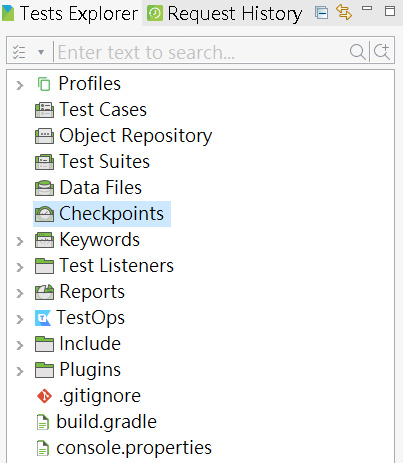
\includegraphics[height=0.75\textheight]{picture/專案結構.jpg}
    \end{columns}
\end{frame}	
%----------------------------
\label{profiles}
\subsection{Profiles}
\begin{frame}[fragile]
    \frametitle{Profiles}
    % -- Code block--
    \begin{block}{Profiles設定值引用}
\begin{lstlisting}
import internal.GlobalVariable
GlobalVariable.varibleName
\end{lstlisting}
    \end{block}
    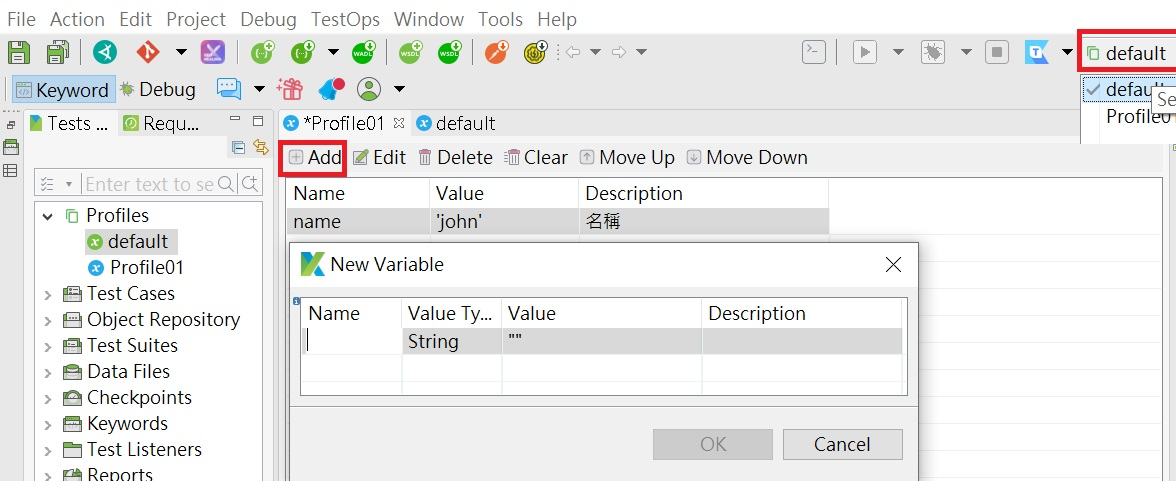
\includegraphics[width=1\textwidth]{picture/Profile新增數值.jpg}
\end{frame}
%----------------------------
\label{objectRepository}
\subsection{Object Repository}
\begin{frame}
    \frametitle{Object Repository}
    Request 物件可以使用變數替代字串方便切環境,寫法為\$\{varibleName\},
    記得切 tab 前要儲存不然已經寫上去的內容會立刻消失。
    %\hyperlink{gstring}{\beamerbutton{gstring}} 
    ~\\
    可以搭配 Profile 中設定的變數做環境設定值切換。
    ~\\~\\
    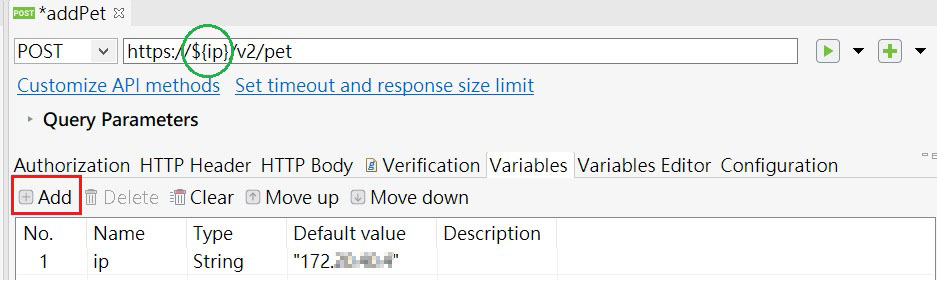
\includegraphics[width=1\textwidth]{picture/addVarible.jpg}
\end{frame}
%----------------------------
\begin{frame}
    \frametitle{Object Repository}
    如果已經有使用 Postman 或者 SoapUI 建立過 Request 也可以直接匯入。
    \begin{center}
        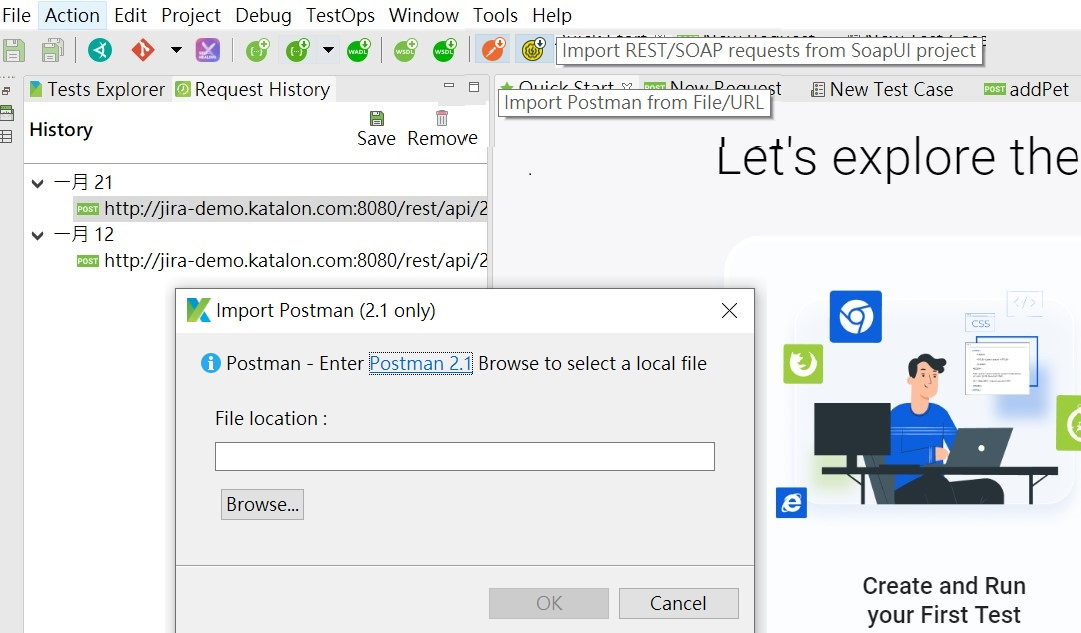
\includegraphics[width=0.9\textwidth]{picture/importRequest.jpg}
    \end{center}
\end{frame}
%----------------------------
\label{dataFile}
\subsection{Data File}
\begin{frame}
	\frametitle{Data Files}
	\begin{block}{測試資料產生的放置位置}
		專案目錄/Data Files/
	\end{block}
	自訂的測試資料檔案(csv/excel)可以不用放這裡,可以設定相對路徑讀取
    \begin{center}
        \includegraphics[width=0.57\textwidth]{picture/example/Data.jpg}
    \end{center}
\end{frame}
%----------------------------
\label{keywords}
\subsection{Keywords}
\begin{frame}
    \frametitle{Keywords}
    所有的自訂 Groovy 類別可以寫在這裡,
    可以直接由 Test Case Script 中直接import使用。
    ~\\~\\
    這裡僅有 Groovy 檔案會顯示出來,
    例如 privateKey.pem 這種檔案就不會顯示,
    但還是可以直接進專案目錄放置該檔案並於Script中讀取。\\
    有讀取 classpath 中檔案需求可以留意。
    ~\\~\\
    如果不是要自訂groovy 類別而是用第三方 library,
    例如:Gson、HikariCP、Jedis ,
    可以將該Jar檔案放到下列目錄裡面就可以使用
    \begin{block}{Library Path}
        專案目錄/Drivers
    \end{block}
\end{frame}
%----------------------------
\label{reports}
\subsection{Reports}
\begin{frame}
    \frametitle{Reports}
    事實上若點擊 Report 功能會提示需要升級的提示,無法直接觀看,
    但仍可以透過輸出報告的方式查看結果,差別僅在不能直接於KatalonStudio中觀看。~\\~\\
    輸出測試結果可以在一個 Test suite 完成後輸出成 Html 檔案。~\\~\\
    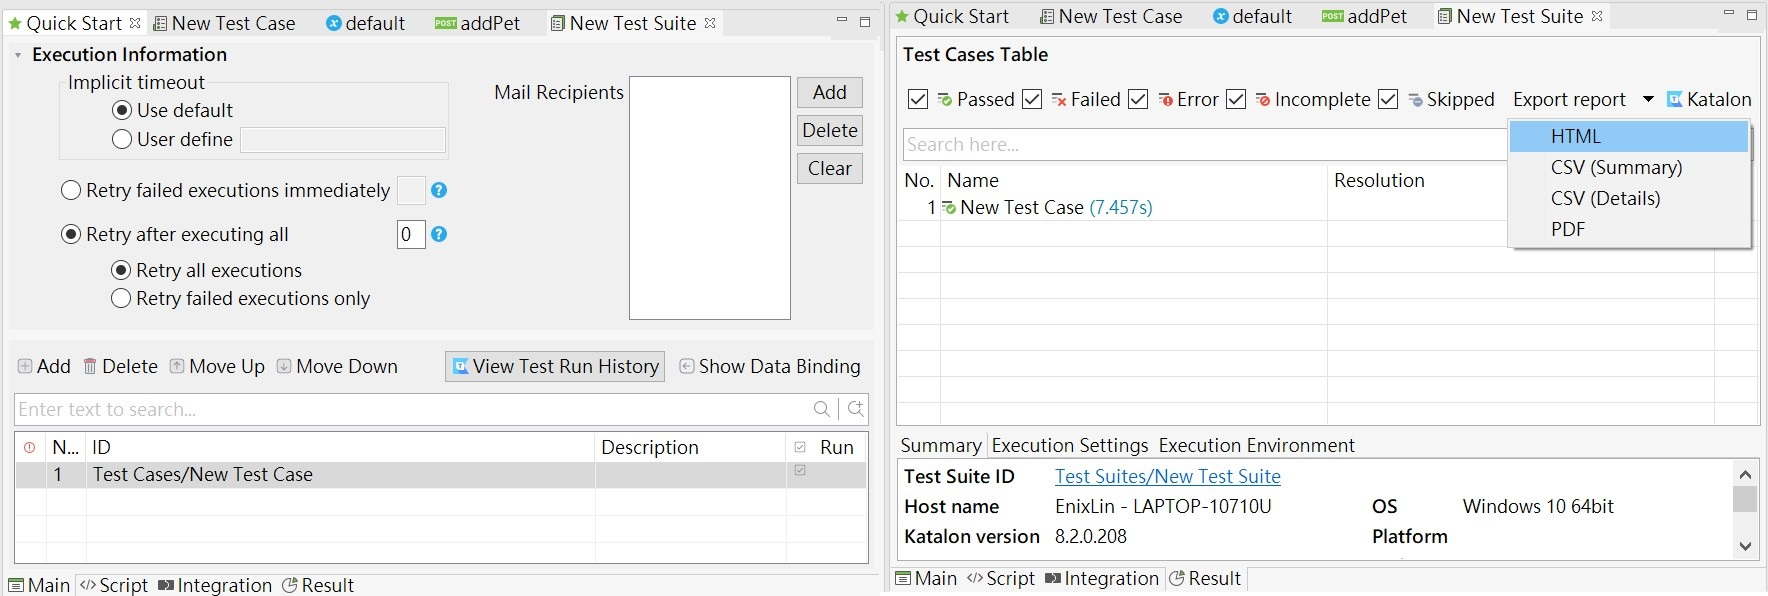
\includegraphics[width=1\textwidth]{picture/輸出報告.jpg}
\end{frame}
%----------------------------
\begin{frame}
    % \frametitle{Reports}
    \begin{center}
        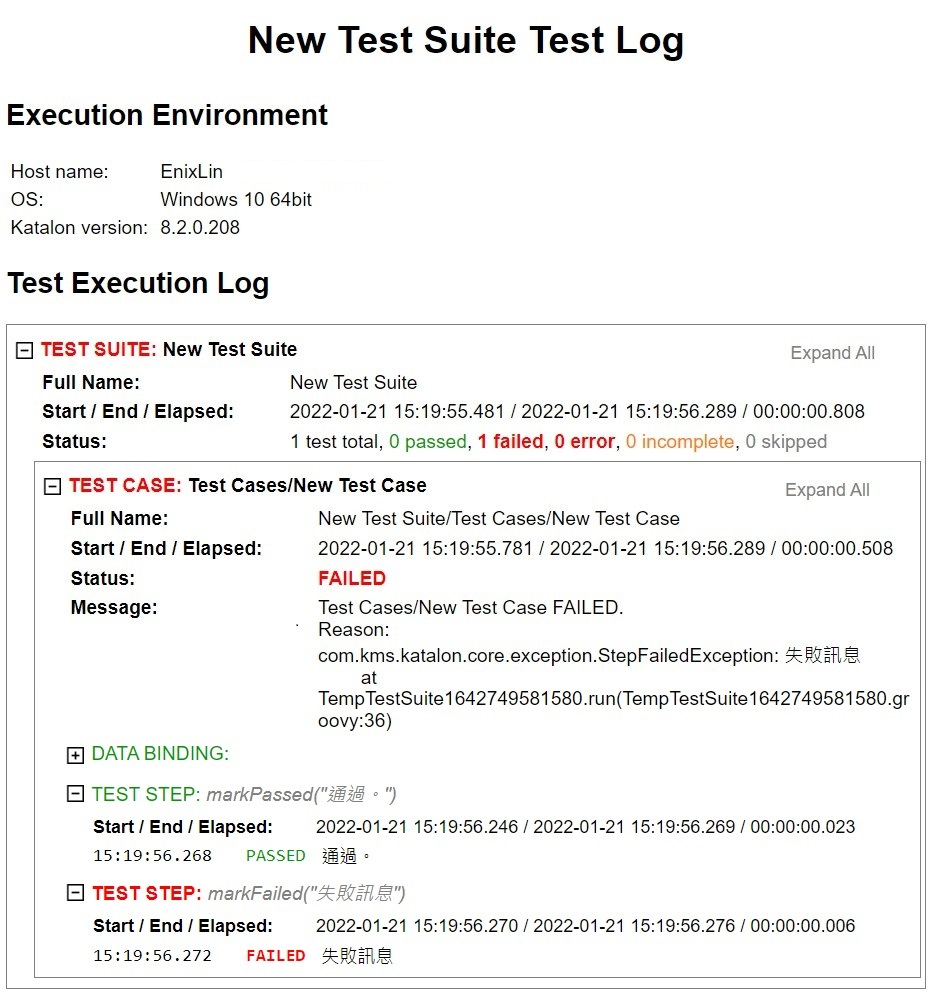
\includegraphics[height=0.95\textheight]{picture/reportHtml.jpg}
    \end{center}
\end{frame}
%----------------------------
\ifx\allfiles\undefined
\end{document}
\fi
	%----------------------------
	% 範例說明
%	\input{example}
	%----------------------------
	% Groovy 介紹
	\ifx\allfiles\undefined
\documentclass{beamer}
\usepackage{xeCJK}
\setmonofont[Mapping={}]{JetBrains Mono}
\setmainfont{JetBrains Mono}
\setsansfont{JetBrains Mono}
\setCJKmainfont{微軟正黑體}
\setCJKsansfont{微軟正黑體}
\usetheme[secheader]{Boadilla}
%\usepackage{ctable} % 表格
\usepackage{color} % 字體顏色
\usepackage{hyperref}
\usepackage{listings} % 程式碼區塊用
\lstset{
	language=Java,
	showtabs=false,
	showstringspaces=false
}
\begin{document}
\input{setting/command}
\fi
%----------------------------
\section{Groovy}
\begin{frame}
  \frametitle{Groovy 介紹}
  Groovy 是 Java 平台上設計的物件導向程式設計語言。
  擁有類似 Python、Ruby 中的一些特性,
  可以作為 Java 平台的 Scripting language 使用,
  Groovy 動態地編譯成執行於 JVM 上的 Java bytecode,
  並與其他 Java code 和 library 進行互操作。由於其執行在JVM上的特性,
  Groovy 可以使用其他 Java 編寫的 Library。~\\~\\
  Groovy 的語法與 Java 非常相似,
  大多數 Java code 也符合 Groovy 的語法規則,
  儘管可能語意不同。~\\
  \begin{center}
    
\includegraphics[width=0.5\textwidth]{picture/Groovy-logo.png}
  \end{center}
\end{frame}
%----------------------------
\subsection{語法知識}
\begin{frame}[fragile]
  \frametitle{變數宣告與方法調用}
  變數可以用 def 關鍵字宣告,所有行句尾不必強制使用分號:
  \begin{block}{宣告一變數}
    def methodName = 'showMessage'
  \end{block}
  如果方法參數只有一個,可以省略其括號,即下列兩行等義:
  \begin{columns}
    \column{.49\textwidth}
    \begin{block}{輸出 Console 1}
      println('Hello World')
    \end{block}
    \column{.49\textwidth}
    \begin{block}{輸出 Console 2}
      println 'Hello World'
    \end{block}
  \end{columns}
  ~\\
  方法可以直接用方法名(String/GString)呼叫:
  \begin{block}{CustomKeywords 物件使用名稱為 verifyResponseErrorCode 的方法}
    CustomKeywords.'verifyResponseErrorCode' (response,'0000')
  \end{block}
\end{frame}
%----------------------------
\begin{frame}[fragile] % 含有 Code 的 frame 要加上 fragile
    \frametitle{Gtring and String}
    以下簡約表示 Gtring 與 String 的不同
    %\hyperlink{objectRepository}{\beamerbutton{objectRepository}}
    % -- Code block--
    \begin{block}{String:單引號}
\begin{lstlisting}
def string = 'this is a string'
\end{lstlisting}
    \end{block}

    % -- Code block--
    \begin{block}{GString:雙引號}
\begin{lstlisting}
def gstring = "hello, ${string}"
println gstring
\end{lstlisting}
    \end{block}
    
    如果使用 println 印出 gstring 變數會顯示 hello, this is a string
\end{frame}
%----------------------------
\begin{frame}[fragile]
  \begin{block}{Script:動態使用方法}
\begin{lstlisting}
def methodName = "showMessage"
def computer = new Computer()
computer."$methodName" "My name is John."
\end{lstlisting}
  \end{block}

  \begin{block}{Class 自訂類別}
\begin{lstlisting}
class Computer {
  void showMessage(def message) {
    println message
  }
}
\end{lstlisting}
  \end{block}
  
  \begin{block}{Console Output}
    My name is John. 
  \end{block}
\end{frame}
%----------------------------
\begin{frame}[fragile]
  \frametitle{List and Map}
  Groovy 有提供快速建立含有資料的 List 與 Map 的語法,使用中括號即可
  快速建立 ArrayList 與 LinkedHashMap 類別。~\\
  搭配 groovy.json.JsonBuilder 可以再轉為 Json 物件。
  \begin{block}{快速建立Map}
\begin{lstlisting}
def map = [
  "key":"value",
  "contractId":"CON0000001",
  "serviceIds":[
    "SVC00001",
    "SVC00002",
    "SVC00003"
  ]
]
\end{lstlisting}
  \end{block}
\end{frame}
%----------------------------
\subsection{實用類別}
\begin{frame}[fragile]
    \frametitle{JsonSlurper / XmlSlurper 類別}
    來自 groovy.json.JsonSlurper / groovy.json.XmlSlurper
    ~\\
    兩個類別可以協助轉換自 WS.sendRequest() 得到的 Response 物件中的內容
    \begin{block}{Sample}
\begin{lstlisting}
ResponseObject response =
  WS.sendRequest(findTestObject('CRMRequest'))
def xmlResult = 
  xmlSlurper.parseText(response.getResponseText())
def jsonResult = 
  jsonSlurper.parseText(xmlResult.text())
def contractId = jsonResult.CONTRACT_ID
\end{lstlisting}
    \end{block}
\end{frame}
%----------------------------
\begin{frame}[fragile]
    \frametitle{Sql 類別}
    來自 groovy.sql.Sql,可以快速建立資料庫連線
    \begin{block}{Sample}
\begin{lstlisting}
def database = Sql.newInstance(
  "jdbcUrl", "userName", "p6d", "driver"
)
def id = "CON01"
def sql = "SELECT * FROM USER WHERE ID = ${id}"
database.eachRow(sql){
  println it.getString("userName")
}
database.close()
\end{lstlisting}
    \end{block}
\end{frame}
%----------------------------
\ifx\allfiles\undefined
\end{document}
\fi

	%----------------------------
	% 參考文件
	\ifx\allfiles\undefined
\documentclass{beamer}
\usepackage{xeCJK}
\setmonofont[Mapping={}]{JetBrains Mono}
\setmainfont{JetBrains Mono}
\setsansfont{JetBrains Mono}
\setCJKmainfont{微軟正黑體}
\setCJKsansfont{微軟正黑體}
\usetheme[secheader]{Boadilla}
%\usepackage{ctable} % 表格
\usepackage{color} % 字體顏色
\usepackage{hyperref}
\usepackage{listings} % 程式碼區塊用
\lstset{
	language=Java,
	showtabs=false,
	showstringspaces=false
}
\begin{document}
\input{setting/command}
\fi
%----------------------------
%----------------------------
\section{Reference}
\begin{frame}
    \frametitle{參考}
    \begin{itemize}
        \item \href{https://docs.groovy-lang.org/docs/next/html/documentation/}{Groovy Language Documentation}
        \item \href{https://qiita.com/opengl-8080/items/a0bb31fb20cb6505188b}{Groovyを知らない人のためのbuild.gradle読み書き入門}
    \end{itemize}
\end{frame}
%----------------------------
\ifx\allfiles\undefined
\end{document}
\fi
	%----------------------------
\end{document}
